

In this chapter we introduce the dynamic system viewpoint of the
optimal planning problem. We restrict the discussion here to
deterministic (rather than stochastic) systems. We consider two
basic settings. The finite-horizon decision problem and its
recursive solution via finite-horizon Dynamic Programming. The
average cost and it related minimum average weight cycle.

\section{Discrete Dynamic Systems}
We consider a discrete-time dynamic system, of the form:
\[{\state_{\ttime + 1}} = {f_{\ttime}}({\state_{\ttime}},{\action_{\ttime}}),\quad \ttime = 0,1,2, \ldots ,\tHorizon - 1\]
where
\begin{itemize}
  \item $\ttime$ is the time index.
  \item ${\state_{\ttime}} \in {\States_{\ttime}}$ is the state variable at time $\ttime$, and $\States_{\ttime}$ is the set of possible states at time
  $\ttime$.
  \item ${\action_{\ttime}} \in {\Actions_{\ttime}}$  is the control variable at time $\ttime$, and $\Actions_{\ttime}$ is the set of possible control actions at time
  $\ttime$.
  \item ${f_{\ttime}}:{\States_{\ttime}} \times {\Actions_{\ttime}} \to {\States_{\ttime + 1}}$ is the state transition function, which defines the \emph{state dynamics} at time
  $\ttime$.
  \item $\tHorizon>0$ is the \emph{time horizon} of the system.  It can be finite or infinite.
\end{itemize}

\begin{remark}
    More generally, the set $\Actions_{\ttime}$ of available actions may depend on the state at time $\ttime$, namely: $\action_{\ttime} \in {\Actions_{\ttime}}({\state_{\ttime}}) \subset
    {\Actions_{\ttime}}$.
\end{remark}
\begin{remark}
The system is, in general, time-varying. It is called \emph{time
invariant} if ${f_{\ttime}},{\States_{\ttime}},{\Actions_{\ttime}}$
do not depend on the time $\ttime$. In that case we
    write
\[{\state_{\ttime + 1}} = f({\state_{\ttime}},{\action_{\ttime}}),\quad \ttime = 0,1,2, \ldots ,\tHorizon - 1;\quad {\state_{\ttime}} \in \States,\;{\action_{\ttime}} \in
\Actions({\state_{\ttime}}).\]
\end{remark}
\begin{remark}
    The state dynamics may be augmented by an output equation:
\[{\observation_{\ttime}} = {\fObservation_{\ttime}}({\state_{\ttime}},{\action_{\ttime}}),\]
where  $\observation_{\ttime}$ is the system observation, or the
output. In most of this book we  implicitly assume that
$\observation_{\ttime}=\state_{\ttime}$, namely, the current state
$\state_{\ttime}$ is fully observed.
\end{remark}

\begin{example}{\textbf{Linear Dynamic Systems}}

A well known example of a dynamic system is that of a linear
time-invariant system, where:
\[{\state_{\ttime + 1}} = A{\state_{\ttime}} + B{\action_{\ttime}}\]
with ${\state_{\ttime}} \in \R^n$, $\action_{\ttime} \in \R^m$,
$A\in\R^{n\times n}$ and $B\in\R^{n\times m}$. Here the state and
action spaces are evidently continuous (and not discrete).
\end{example}

\begin{example}{\textbf{Finite models}}

Our emphasis here will be on \emph{finite state and action} models.
A finite state space contains a finite number of points:
${\States_{\ttime}} = \{ 1,2, \ldots ,{n_{\ttime}}\} $. Similarly, a
finite action space implies a finite number of control actions at
each stage:
\[{\Actions_{\ttime}}(\state) = \{ 1,2, \ldots ,{m_{\ttime}}(\state)\} ,\;\;\state \in {\States_{\ttime}}\]
\end{example}

%\paragraph{Notation for finite models:}
%When the state and action spaces are finite, it is common to denote
%the state by ${s_{\ttime}}$ (instead of ${x_{\ttime}}$) and the
%actions by ${\action_{\ttime}}$ (instead of ${u_{\ttime}}$). That is, the
%system equations are written as: ${s_{k + 1}} =
%{f_{\ttime}}({s_{\ttime}},{\action_{\ttime}}),\quad k = 0,1,2, \ldots ,N -
%1$ with ${s_{\ttime}} \in {S_{\ttime}}$, ${\action_{\ttime}} \in
%{A_{\ttime}}({x_{\ttime}}) \subset {A_{\ttime}}$. \textbf{We will
%adhere to that notation in the following}.


\paragraph{Graphical description:} Finite models (over finite time horizons) can be represented by a corresponding decision graph:

\begin{centering}
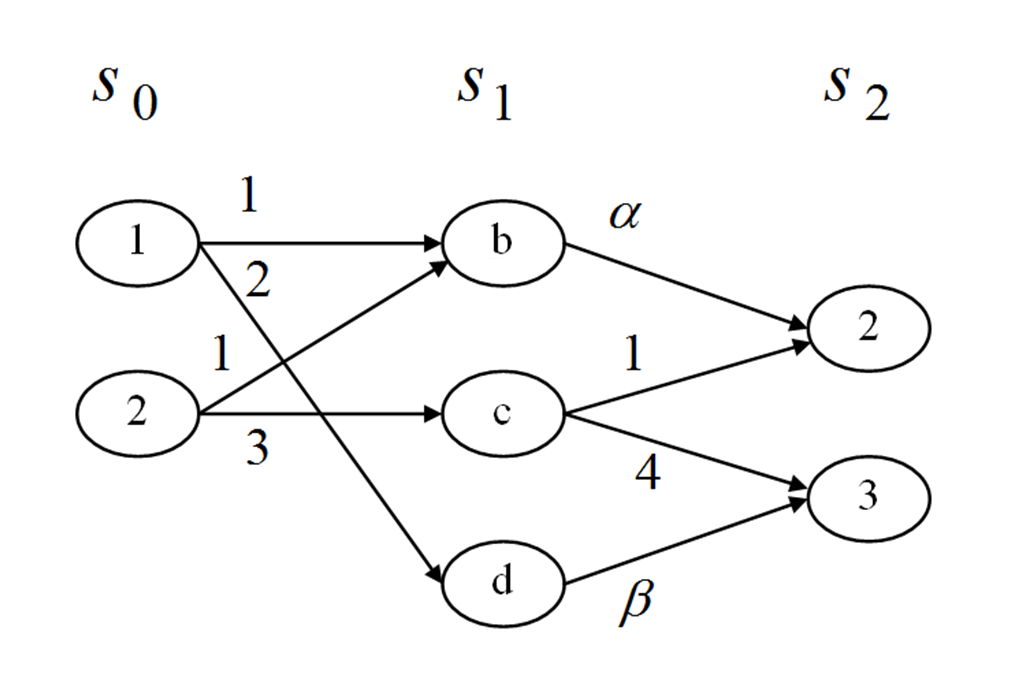
\includegraphics[width=0.5\textwidth]{figures/lecture2_decision_graph.png}\\
\end{centering}

Here:
\begin{itemize}
  \item $\tHorizon = 2$, ${\States_0} = \{ 1,2\} ,\;{\States_1} = \{ b,c,d\} ,\;{\States_2} = \{ 2,3\} $,
  \item ${\Actions_0}(1) = \{ 1,2\} $, ${\Actions_0}(2) = \{ 1,3\} $, ${\Actions_1}(b) = \{ \alpha \} $, ${\Actions_1}(c) = \{ 1,4\} $, ${\Actions_1}(d) = \{ \beta \} $
  \item ${f_0}(1,1) = b,\;{f_0}(1,2) = d,\;{f_0}(2,1) = b,\;{f_0}(2,3) = c$, ${f_1}(b,\alpha ) = 2$, etc.
\end{itemize}

\begin{definition}{\textbf{Feasible Path}} \\
A feasible path for the specified system is a sequence
$({\state_0},{\action_0}, \ldots ,{\state_{\tHorizon -
1}},{\action_{\tHorizon - 1}},{\state_\tHorizon})$ of states and
actions, such that ${\action_{\ttime}} \in
{\Actions_{\ttime}}({\state_{\ttime}})$ and ${\state_{\ttime + 1}} =
{f_{\ttime}}({\state_{\ttime}},{\action_{\ttime}})$.

%\vspace{10pt}
\bigskip

\begin{centering}
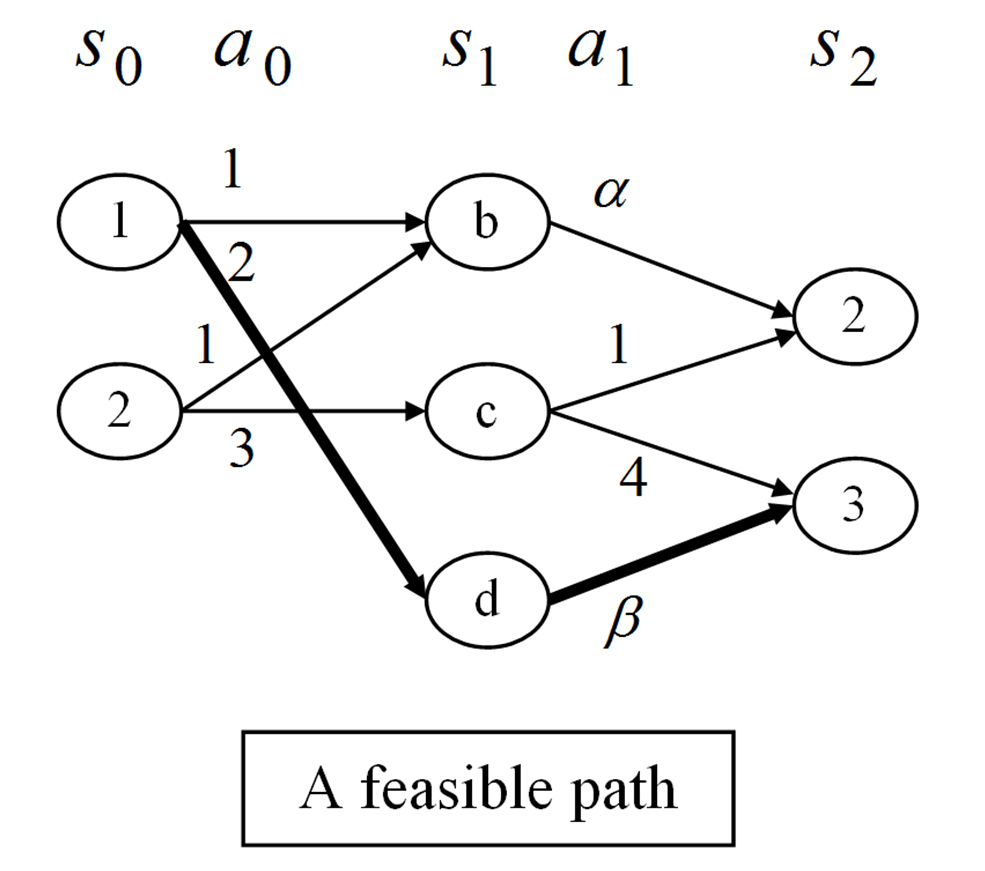
\includegraphics[width=0.4\textwidth]{figures/lecture2_feasible_path}\\
\end{centering}
\end{definition}

\section{The Finite Horizon Decision Problem}

We proceed to define our first and simplest planning problem. For
that we need to specify a \emph{performance objective} for our
model, and the notion of \emph{control policies}.

\subsection{Costs and Rewards}

\paragraph{The cumulative cost:}
Let ${\thistory_\tHorizon} = ({\state_0},{\action_0}, \ldots
,{\action_{\tHorizon - 1}},{\state_{\tHorizon -
1}},{\state_\tHorizon})$ denote a $\tHorizon$-stage feasible path
for the system. Each feasible path ${\thistory_\tHorizon}$ is assigned
some cost ${\Cost_\tHorizon} =
{\Cost_\tHorizon}({\thistory_\tHorizon})$.

The standard definition of the cost ${\Cost_\tHorizon}$ is through
the following \emph{cumulative cost functional}:
\[{\Cost_\tHorizon}({\history_\tHorizon}) = \sum_{\ttime = 0}^{\tHorizon - 1} {{\cost_{\ttime}}({\state_{\ttime}},{\action_{\ttime}}) + {c_\tHorizon}({\state_\tHorizon})} \]

Here:
    \begin{itemize}
    \item
${\cost_{\ttime}}({\state_{\ttime}},{\action_{\ttime}})$ is the
\emph{instantaneous}  cost or \emph{single-stage }cost at stage
$\ttime$, and ${\cost_{\ttime}}$ is the instantaneous cost function.
    \item
${\cost_\tHorizon}({\state_\tHorizon})$ is the \emph{terminal} cost,
and ${\cost_\tHorizon}$ is the terminal cost function.
  \end{itemize}

\paragraph{Note:}
\begin{itemize}
  \item The cost functional defined above is \emph{additive} in time. Other cost functionals are possible, for example the max cost, but additive cost is by far the most common and useful.
  \item We shall refer to ${\Cost_\tHorizon}$ as the \emph{cumulative $\tHorizon$-stage cost}, or just the \emph{cumulative cost}.
\end{itemize}

Our objective is to \emph{minimize} the cumulative cost
${\Cost_\tHorizon}$, by a proper choice of actions. We will define
that goal more formally in the next section.

\paragraph{Cost versus reward formulation: }
It is often more natural to consider \emph{maximizing} reward rather
than minimizing cost.  In that case, we define the cumulative
$\tHorizon$-stage return function:
$${\Value_\tHorizon}({h_\tHorizon}) = \sum_{\ttime = 0}^{\tHorizon - 1} {{\reward_{\ttime}}({\state_{\ttime}},{\action_{\ttime}}) + {\reward_\tHorizon}({\state_\tHorizon})} $$
Here, ${\reward_{\ttime}}$ is the instantaneous reward and
${\reward_\tHorizon}$ is the terminal reward. Clearly, minimizing
${\Cost_\tHorizon}$ is equivalent to maximizing
${\Value_\tHorizon}$, if we set:
$${\reward_{\ttime}}(\state,\action) =  - {\cost_{\ttime}}(\state,\action) \text{ and }{\reward_\tHorizon}(\state) =  - {\cost_\tHorizon}(\state).$$

We denote by $\T$ the set of time steps for horizon $\tHorizon$, i.e.,
$\T=\{1, \ldots, \tHorizon\}$


\subsection{Optimal Paths}

Our first planning problem is the following \emph{$\tHorizon$-stage
Finite Horizon Problem}:
\begin{itemize}
\item For a given initial state ${\state_0}$, find a feasible path
  ${\history_\tHorizon} = ({\state_0},{\action_0}, \ldots ,{\state_{\tHorizon - 1}},{\action_{\tHorizon - 1}},{\state_\tHorizon})$
  that minimizes the cost functional ${\Cost_\tHorizon}({\history_\tHorizon})$, over all feasible paths ${\history_\tHorizon}$.
\end{itemize}
%
Such a feasible path ${\history_\tHorizon}$ is called an
\emph{optimal path} from ${\state_0}$.

A more general notion than a path is that of a \emph{control
policy}, that specifies the action to be taken at each state.
Control policies will play an important role in our Dynamic
Programming algorithms, and are defined next.

\subsection{Control Policies}
%%%%%%%%%%%%%%%%%%%%%%

In general we will consider a few classes of control policies. The
two basic dimensions in which we will characterize the control
policies is their dependence on the history, and their use of
randomization.


\begin{itemize}
\item
A general or \textbf{history-dependent} control policy $\policy  =
{({\policy _\ttime})_{\ttime \in \T}}$ is a mapping from each
possible history ${\history_\ttime} = ({\state_0},{\action_0},
\ldots ,{\state_{\ttime-1}},{\action_{\ttime-1}},{\state_\ttime})$,
$\ttime \in \T$, to an action ${\action_\ttime} = {\policy
_\ttime}({\history_\ttime}) \in {\Actions_\ttime}$.  We denote the
set of general policies by ${\Pi _H}$.
%
\item
A \textbf{Markov} control policy $\policy $ is allowed to depend on
the current state and time only: ${\action_\ttime} = {\policy
_\ttime}({\state_\ttime})$.   We denote the set of Markov policies
by ${\Pi _M}$.
%
\item
For stationary models, we may define \textbf{stationary} control
policies that depend on the current state alone. A stationary policy
is defined by a single mapping $\policy :\States \to \Actions$, so
that ${\action_\ttime} = \policy ({\state_\ttime})$ for all $\ttime
\in \T$. We denote the set of stationary policies by ${\Pi _S}$.
%
\item
Evidently, ${\Pi _H} \supset {\Pi _M} \supset {\Pi _S}$.
\end{itemize}

\paragraph{Randomized (Stochastic) Control policies}
\begin{itemize}
  \item The control policies defined above specify deterministically the action to be taken at each stage. In some cases we want to allow for a random choice of action.
  \item
A general randomized (stochastic) control policy assigns to each
possible history ${\history_\ttime}$ a probability distribution
${\policy _\ttime}( \cdot |{\history_\ttime})$ over the action set
${\Actions_\ttime}$. That is,  $\Pr\{ {\action_\ttime} =
\action|{\history_\ttime}\}  = {\policy
_\ttime}(\action|{\history_\ttime})$. We denote the set of general
randomized policies by ${\Pi _{HS}}$.
  \item Similarly, we can define the set ${\Pi _{MS}}$ of Markov randomized (stochastic) control policies, where ${\policy _\ttime}( \cdot |{\history_\ttime})$ is replaced by ${\policy _\ttime}( \cdot |{\state_\ttime})$, and the set ${\Pi _{SS}}$ of stationary randomized (stochastic) control policies, where ${\policy _\ttime}( \cdot |{\state_\ttime})$ is replaced by  $\policy ( \cdot |{\state_\ttime})$.
  \item Note that the set ${\Pi _{HS}}$ includes all other policy sets as special cases.
  \item For deterministic control policies, we similarly define ${\Pi _{HD}} \supset {\Pi _{MD}} \supset {\Pi _{SD}}$
\end{itemize}


%%%%%%%%%%%%%%%%%%%%%

%\begin{definition}
%A control policy, denoted $\policy $, specifies for each state a unique
%action to be taken at this state. Specifically, a control policy
%$\policy $ is a sequence $\policy  = ({\policy _0}, \ldots ,{\policy _{N - 1}})$ of
%decision functions, where ${\policy _{\ttime}}:{\States_{\ttime}} \to {\Actions_{\ttime}}$,    and  ${\policy
%_{\ttime}}(s) \in {\Actions_{\ttime}}(s)$. The action to be taken at time $k$ in state
%${\state_{\ttime}}$ is given as ${\action_{\ttime}} = {\policy _{\ttime}}({\state_{\ttime}})$
%\end{definition}
%
%\paragraph{Classes of control policies}
%Observe that we allow the function ${\policy _{\ttime}}$ policy to depend on
%the time $k$. Such time-dependent policies are also called
%\emph{non-stationary}. On the other hand, we confine ourselves here
%to policies that are:
%\begin{itemize}
%  \item \textbf{Markovian}: The action ${\action_{\ttime}}$ is a function of the current state ${\state_{\ttime}}$ only, and not on previous states and actions. Non-Markovian policies: also called history-dependent policies, will be extensively used in the learning part of the course.
%  \item \textbf{Deterministic}: More general policies may use randomization in the selection of actions. Such randomized policies are also used in learning algorithms, as well as in game problems.
%\end{itemize}

\paragraph{Control policies and paths:}
As mentioned, a control policy specifies an action for each state,
whereas a path specifies an action only for states along the path.
The definition of a policy, allows us to consider counter-factual
events, namely, what would have been the path if we considered a
different action. This distinction is illustrated in the following
figure.

\begin{centering}
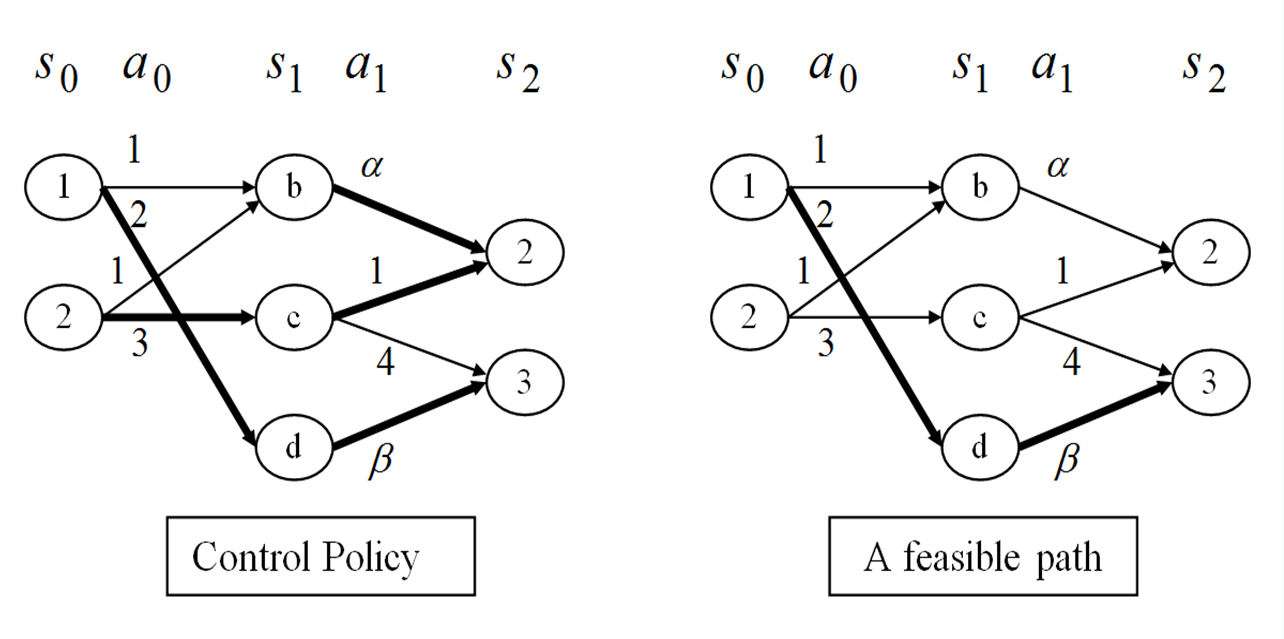
\includegraphics[width=0.8\textwidth]{figures/lecture2_policy_path}\\
\end{centering}

\paragraph{Induced Path:}
A control policy $\policy $, together with an initial state
${\state_0}$, specify a feasible path ${\history_\tHorizon} =
({\state_0},{\action_0}, \ldots ,{\state_{N -
1}},{\action_{\tHorizon - 1}},{\state_\tHorizon})$. This path may be
computed recursively using ${\action_{\ttime}} = {\policy
_{\ttime}}({\state_{\ttime}})$ and ${\state_{\ttime + 1}} =
{f_{\ttime}}({\state_{\ttime}},{\action_{\ttime}})$, for $\ttime =
0,1, \ldots ,\tHorizon - 1$.

\begin{remark}
Suppose that for each state ${\state_{\ttime}}$, each action
${\action_{\ttime}} \in {\Actions_{\ttime}}({\state_{\ttime}})$
leads to a different state ${\state_{\ttime + 1}}$ (i.e., at most
one edge connects any two states). We can then identify each action
${\action_{\ttime}} \in {\Actions_{\ttime}}(\state_{\ttime})$ with
the next state ${\state_{\ttime + 1}} =
{f_{\ttime}}(\state_{\ttime},{\action_{\ttime}})$ it induces. In
that case a path may be uniquely specified by the state sequence
$({\state_0},{\state_1}, \ldots ,{\state_\tHorizon})$.
\end{remark}

%\newpage

\subsection{Reduction between control policies classes}

We first show a reduction from a general history dependent policies
to Randomized Markovian policies. The main observation is that the
only influence on the cumulative cost is the expected instantaneous
cost $\E[\cost_\ttime(\state_\ttime,\action_\ttime)]$. Namely, let
\[
\rho^\policy_\ttime(\state,\action)=\Pr_{\history'_{\ttime-1}}
[\action_\ttime=\action,\state_\ttime=\state]=\E_{\history'_{\ttime-1}}[\I
[\state_\ttime=\state,\action_\ttime=\action]| \history'_{\ttime-1}],
\]
where
$\history'_{\ttime-1}=(\state_0,\action_0,\ldots,\state_{t-1},\action_{t-1})$
is the history of the first $\ttime-1$ time steps generated using
$\policy$, and the probability and expectation are taken with
respect to the randomness of the policy $\policy$. Now we can
rewrite the expected cost to go as,
\[
\E[\Cost^\policy(\state_0)]=\sum_{\ttime=0}^{\tHorizon-1}
\sum_{\action\in \Actions_\ttime,\state\in \States_\ttime}
\cost_\ttime(\state,\action)\rho^\pi_\ttime(\state,\action),
\]
where $\Cost^\policy(\state_0)$ is the random variable of the cost
when starting at state $\state_0$ and following policy $\policy$.

This implies that any two policies $\policy$ and $\policy'$ for
which
$\rho^\policy_\ttime(\state,\action)=\rho^{\policy'}_\ttime(\state,\action)$,
for any time $\ttime$, state $\state$ and action $\action$, would
have the same expected cumulative cost for any cost function, i.e.,
$\E[\Cost^\policy(\state_0)]=\E[\Cost^{\policy'}(\state_0)]$

% we need to show that we can preserve the probabilities
%$\rho^\policy_\ttime(\state,\action)$.

%\newpage

\begin{theorem}
\label{chp2:HS-MS}
For any policy $\policy\in \Pi_{HS}$, there is a policy
$\policy'\in\Pi_{MS}$, such that for every state $\state$ and action
$\action$ we have,
$\rho^{\policy}(\state,\action)=\rho^{\policy'}(\state,\action)$.
This will imply that,
\[
\E[\Cost^\policy(\state_0)]=\E[\Cost^{\policy'}(\state_0)]
\]
\end{theorem}

\begin{proof}
Given the policy  $\policy\in \Pi_{HS}$, we define
$\policy'\in\Pi_{MS}$ as follows. For every state $\state\in
\States_\ttime$ we define
\[
\policy'_\ttime(\action|\state)=\Pr_{\history_{\ttime-1}}
[\action_\ttime=\action|\state_\ttime=\state]=\frac{\rho^\policy_\ttime(\state,\action)}{\sum_{\action'\in
\Actions_\ttime} \rho^\policy_\ttime(\state,\action')}
\]
By definition $\policy'$ is Markovian (depends only on the time
$\ttime$ and the realized state $\state$). By construction
$\rho_\ttime^{\policy}(\state,\action)=\rho_\ttime^{\policy'}(\state,\action)$
is identical, which implies that
$\E[\Cost^\policy(\state_0)]=\E[\Cost^{\policy'}(\state_0)]$.
\end{proof}

Next we show that for any stochastic Markovian policy there is a
deterministic Markovian policy with at most the same cumulative
cost.

\begin{theorem}
\label{chp2:stochastic-deterministic}
For any policy $\policy\in \Pi_{MS}$, there is a policy
$\policy'\in\Pi_{MD}$, such that
\[
\E[\Cost^\policy(\state_0)]\geq \E[\Cost^{\policy'}(\state_0)]
\]
\end{theorem}

\begin{proof}
The proof is by backward induction on the steps. The inductive claim is:\\
{\em For any policy $\policy\in \Pi_{MS}$ which is deterministic in
$[\ttime+1,\tHorizon]$, there is a policy $\policy'\in \Pi_{MS}$
which is deterministic in $[\ttime,\tHorizon]$ and
$\E[\Cost^\policy(\state_0)]\geq
\E[\Cost^{\policy'}(\state_0)]$.}\\
Clearly, the theorem follows from the case of $\ttime=0$.

For the base of the induction we can take $\ttime=\tHorizon$, which
holds trivially.

For the inductive step, assume that $\policy\in \Pi_{MS}$ is
deterministic in $[\ttime+1,\tHorizon]$.

%For the proof, it would be useful to introduce
%$path^\policy_\ttime(\state)=(\state_\ttime, \ldots ,
%\state_\tHorizon)$, where $\state_\ttime=\state$ and
%$\state_{\ttime+i+1}=\policy_{\ttime+i}(\state_{\ttime+i})$.

For every $\state_{\ttime+1}\in \States_{\ttime+1}$ define
\[
\Cost_{\ttime+1}(\state_{\ttime+1})=\Cost(path(\state_{\ttime+1},
\dots , \state_\tHorizon)),
\]
where $path(\state_{\ttime+1}, \dots , \state_\tHorizon)$ is the
deterministic path from $\state_{\ttime+1}$ induced by $\policy$.

We define $\policy'$ to be identical to $\policy$ for all time steps
$\ttime'\neq \ttime$. We define $\policy'_\ttime$ for each
$\state_\ttime\in \States_\ttime$ as follows:
\begin{equation}
\label{eq:sec2-MS-MD}
\policy'_\ttime(\state_\ttime)=\arg\min_{\action\in
\Actions_\ttime} \cost_{\ttime}(\state_\ttime,\action)+
\Cost_{\ttime+1}(f_\ttime(\state_\ttime,\action)).
\end{equation}
Recall that since we have a Deterministic Decision Process
$f_\ttime(\state_\ttime,\action_\ttime)\in \States_{\ttime+1}$ is
the next state if we take action $\action$ in $\state_\ttime$.
%(Remark: For a stochastic $f_\ttime$ we would simply take the expectation.)

For the analysis, note that $\policy$ and $\policy'$ are identical
until time $\ttime$, so they generate exactly the same distribution
over paths. At time $\ttime$, $\policy'$ is defined to minimize the
cost to go from $\state_\ttime$, given that we follow $\policy$ from
$\ttime+1$ to $\tHorizon$. Therefore the cost can only decrease.
Formally, let $\E^\policy[\cdot]$ be the expectation with respect to
policy $\policy$.
\begin{align*}
\E^\policy_{\state_\ttime}[\Cost_{\ttime}(\state_\ttime)]
%=\E^\policy[\Cost(\state_\ttime, \ldots , \state_\tHorizon)]
= & \E^\policy_{\state_\ttime}
\E^\policy_{\action_\ttime}[\cost_{\ttime}(\state_\ttime,\action_\ttime)+\Cost_{\ttime+1}(f_\ttime(\state_\ttime,\action_\ttime))]\\
\geq & \E^\policy_{\state_\ttime} \min_{\action_\ttime\in
\Actions_\ttime}[\cost_{\ttime}(\state_\ttime,\action_\ttime)+\Cost_{\ttime+1}(f_\ttime(\state_\ttime,\action_\ttime))]\\
= & \E^{\policy'}_{\state_\ttime} [\Cost_\ttime (\state_\ttime)]
\end{align*}
which completes the inductive proof.
%
%\begin{align*}
%\E[\Cost^\policy_{\tHorizon-\ttime}]=\E[\Cost(\state_\ttime, \ldots
%, \state_\tHorizon)]=& \E^\policy
%\E_{\action_\ttime}[\Cost(f_\ttime(\state_\ttime,\action_\ttime),
%\state_{\ttime+1},
%\ldots ,\state_\tHorizon)]\\
%\geq& E^\policy \min_{\action_\ttime\in
%\Actions_\ttime}[\Cost(f_\ttime(\state_\ttime,\action_\ttime),
%\state_{\ttime+1},
%\ldots ,\state_\tHorizon)]\\
%=&\E^{\policy'} [\Cost(f_\ttime(\state_\ttime,\action_\ttime),
%\state_{\ttime+1}, \ldots ,\state_\tHorizon)]
%\end{align*}
\end{proof}

\begin{remark}
The above proof extends very naturally for the case of a stochastic
MDP, which implies that $f_\ttime$ is stochastic. The modification
of the proof would simply take the expectation over $f_\ttime$ in
Eq. \ref{eq:sec2-MS-MD}.
\end{remark}



\subsection{Optimal Control Policies}

\begin{definition}
A control policy $\policy\in\Pi_{MD} $ is called \textbf{optimal}
if, for each initial state ${\state_0}$, it induces an optimal path
${\history_\tHorizon}$ from ${\state_0}$.
\end{definition}

An alternative definition can be given in terms of policies only.
For that purpose, let ${\history_\tHorizon}(\policy ;{\state_0})$
denote the path induced by the policy $\policy $ from ${\state_0}$.
For a given return functional
${\Value_\tHorizon}({\history_\tHorizon})$, denote
${\Value_\tHorizon}(\policy ;{\state_0}) =
{\Value_\tHorizon}({\history_\tHorizon}(\policy ;{\state_0}))$ That
is, ${\Value_\tHorizon}(\policy ;{\state_0})$ is the cumulative
return for the path induced by $\policy $ from ${\state_0}$.

\begin{definition}
A control policy $\policy \in\Pi_{MD}$ is called optimal if, for
each initial state ${\state_0}$, it holds that
${\Value_\tHorizon}(\policy ;{\state_0}) \ge
{\Value_\tHorizon}(\tilde \policy ;{\state_0})$ for any other policy
$\tilde \policy \in\Pi_{MD}$.
\end{definition}

Equivalence of the two definitions can be easily established
(exercise). An optimal policy is often denoted by ${\policy ^*}$.

\vspace{10pt} \fbox{\begin{minipage}{0.9\textwidth} \textbf{The
standard $\tHorizon$-stage finite-horizon planning problem:}  Find a
control policy $\policy $ for the $\tHorizon$-stage Finite Horizon
problem that minimizes the cumulative cost (or maximizes the
cumulative return) function.
\end{minipage}}


\normalsize
\paragraph{The naive approach to finding an optimal policy:}
For finite models (i.e., finite state and action spaces), the number
of feasible paths (or control policies) is finite.  It is therefore
possible, in principle, to enumerate all $\tHorizon$-stage paths,
compute the cumulative return for each one, and choose the one which
gives the largest return. Let us evaluate the number of different
paths and control policies. Suppose for simplicity that number of
states at each stage is the same: $|{\States_{\ttime}}| = n$, and
similarly the number of actions at each state is the same:
$|{\Actions_{\ttime}}(\state)| = m$ (with $m \le n$) . The number of
feasible $\tHorizon$-stage paths for each initial state is seen to
be ${m^\tHorizon}$. The number of different policies is
${m^{n\tHorizon}}$. For example, for a fairly small problem with
$\tHorizon = n = m = 10$, we obtain ${10^{10}}$ paths for each
initial state (and ${10^{11}}$ overall), and ${10^{100}}$ control
policies. Clearly it is not computationally feasible to enumerate
them all.

Fortunately, Dynamic Programming offers a drastic reduction of the
computational complexity for this problem.

\section{Finite Horizon Dynamic Programming}

The Dynamic Programming (DP) algorithm breaks down the
$\tHorizon$-stage finite-horizon problem into $\tHorizon$ sequential
single-stage optimization problems. This results in dramatic
improvement in computation efficiency.

The DP technique for dynamic systems is based on a general
observation called Bellman's Principle of Optimality. Essentially, it
states the following (for deterministic problems):
\begin{itemize}
  \item \textbf{Any sub-path of an optimal path is itself an optimal path between its end points.}
\end{itemize}
To see why this should hold, consider a sub-path which is not
optimal. We can replace it by an optimal sub-path, and improve the
return.

Applying this principle recursively from the last stage backward,
obtains the (backward) Dynamic Programming algorithm. Let us first
illustrate the idea with following example.

\begin{example}
Shortest path on a decision graph:  Suppose we wish to find the
shortest path (minimum cost path) from the initial node in
$\tHorizon$ steps.

\begin{centering}
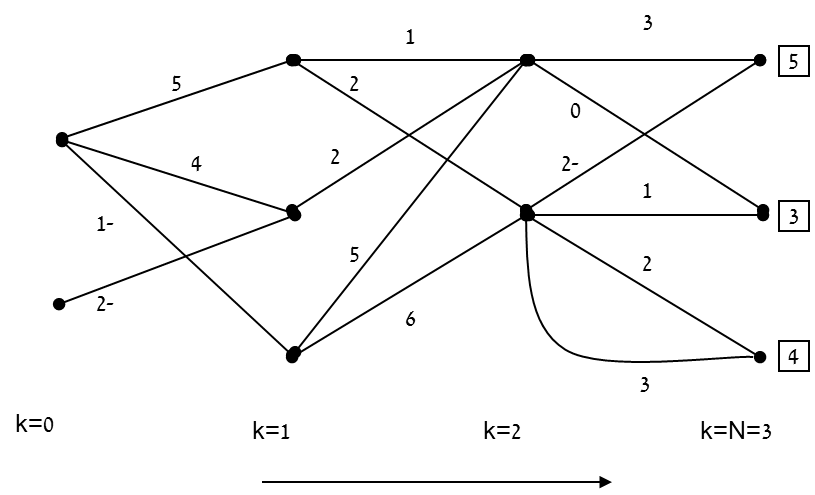
\includegraphics[width=0.8\textwidth]{figures/lecture2_DP}
\end{centering}

\medskip
The boxed values are the terminal costs at stage $\tHorizon$, the
other number are the link costs. Using backward recursion, we may
obtain that the minimal path costs from the two initial states are
$7$ and $3$, as well as the optimal paths and an optimal policy.
\end{example}

We can now describe the DP algorithm. Recall that we consider the dynamic system
$${\state_{\ttime + 1}} = {f_{\ttime}}({\state_{\ttime}},{\action_{\ttime}}),\quad \ttime = 0,1,2, \ldots ,\tHorizon - 1$$
$${\state_{\ttime}} \in {\States_{\ttime}},\quad {\action_{\ttime}} \in {\Actions_{\ttime}}({\state_{\ttime}})$$
and we wish to maximize the cumulative return:
$${\Value_\tHorizon} = \sum_{\ttime = 0}^{\tHorizon - 1} {{\reward_{\ttime}}({\state_{\ttime}},{\action_{\ttime}}) + {\reward_\tHorizon}({\state_\tHorizon})} $$
The DP algorithm computes recursively a set of \textbf{value
functions} $\Value_{\ttime}^{}:{\States_{\ttime}} \to \R$ , where
$\Value_{\ttime}^{}({\state_{\ttime}})$ is the value of an optimal
sub-path ${\history_{\ttime:\tHorizon}} =
({\state_{\ttime}},{\action_{\ttime}}, \ldots ,{\state_\tHorizon})$
that starts at ${\state_{\ttime}}$.

%\begin{algorithm_}
%\label{Alg:FHDP-DDP} \textbf{Finite-horizon Dynamic Programming}
%\begin{enumerate}
%  \item Initialize the value function:  $\Value_\tHorizon(\state) = {\reward_\tHorizon}(\state)$,  $\state \in {\States_\tHorizon}$.
%  %$V_N^{}(s) = {r_N}(s)$,  $s \in {S_N}$.
%  \item Backward recursion:  For $\ttime = \tHorizon - 1, \ldots ,0$, compute
%%\[V_k^{}(s) = \mathop {\max }\limits_{a \in {A_k}} \left\{ {{r_k}(s,a) + V_{k + 1}^{}({f_k}(s,a))} \right\},\quad     s \in {S_k}.\]
%\[\Value_{\ttime}^{}(\state) = \mathop {\max }\limits_{\action \in {\Actions_{\ttime}}} \left\{ {{\reward_{\ttime}}(\state,\action) + \Value_{\ttime + 1}^{}({f_{\ttime}}(\state,\action))} \right\},\quad     \state \in {\States_{\ttime}}.\]
%  \item Optimal policy: Choose any control policy $\policy^*  = ({\policy^* _{\ttime}})$ that satisfies:
%%\[\pi _k^{}(s) \in \mathop {\arg \max }\limits_{a \in {A_k}} \left\{ {{r_k}(s,a) + V_{k + 1}^{}({f_k}(s,a))} \right\},\quad k = 0, \ldots ,N - 1.\]
%\[\policy^* _{\ttime}(\state) \in \mathop {\arg \max }\limits_{\action \in {\Actions_{\ttime}}} \left\{ {{\reward_{\ttime}}(\state,\action) + \Value_{\ttime + 1}^{}({f_{\ttime}}(\state,\action))} \right\},\quad \ttime = 0, \ldots ,\tHorizon - 1.\]
%\end{enumerate}
%\end{algorithm_}

\begin{algorithm_}
\label{Alg:FHDP-DDP} \textbf{Finite-horizon Dynamic Programming}
\begin{enumerate}
  \item Initialize the value function:
  $\Value_\tHorizon(\state) = {\reward_\tHorizon}(\state)$,  $\state \in {\States_\tHorizon}$.
  \item Backward recursion:  For $\ttime = \tHorizon - 1, \ldots ,0$, compute
\[\Value_{\ttime}^{}(\state) = \mathop {\max }\limits_{\action \in {\Actions_{\ttime}}} \left\{ {{\reward_{\ttime}}(\state,\action) + \Value_{\ttime + 1}^{}({f_{\ttime}}(\state,\action))} \right\},\quad     \state \in {\States_{\ttime}}.\]
  \item Optimal policy: Choose any control policy $\policy^*  = ({\policy^* _{\ttime}})$ that satisfies:
\[\policy^* _{\ttime}(\state) \in \mathop {\arg \max }\limits_{\action \in {\Actions_{\ttime}}} \left\{ {{\reward_{\ttime}}(\state,\action) + \Value_{\ttime + 1}^{}({f_{\ttime}}(\state,\action))} \right\},\quad \ttime = 0, \ldots ,\tHorizon - 1.\]
\end{enumerate}
\end{algorithm_}

\begin{proposition}
The following holds for finite-horizon dynamic programming:
\begin{enumerate}
  \item
The control policy $\policy^* $ computed in Algorithm
\ref{Alg:FHDP-DDP} (Finite-horizon Dynamic Programming) is an optimal control policy for the
$\tHorizon$-stage Finite Horizon problem.
  \item $\Value_0^{}(\state)$ is the optimal $\tHorizon$-stage return from initial state ${\state_0} = \state$:
\[{\Value_0}(s) = \mathop {\max }\limits_\policy  {\Valuepi_0}(\state),\;\quad \forall \state \in {\States_0},\]
where $\Valuepi_0(\state)$ is the expected return of policy $\pi$
when started at state $\state$.
\end{enumerate}
\end{proposition}

\begin{proof}
We show that the computed policy $\policy^*$ is optimal and its
return from time $\ttime$ is $\Value_{\ttime}$. We will establish
the following inductive claim:

\smallskip
\noindent{\em For any time $\ttime$ and any state $\state$, the path
from $\state$ defined by $\policy^*$ is the maximum return path of
length $\tHorizon-\ttime$. The value of $\Value_\ttime (\state)$ is
the maximum return from $\state$.}

\smallskip
The proof is by a backward induction. For the basis of the induction
we have: $\ttime=\tHorizon$, and the inductive claim follows from
the initialization.

%Assume the inductive claim holds for $\ttime$ prove for $\ttime+1$.
%For contradiction assume there is a lower cost path from $\state$.
%Let the path generated $\policy^*$ be
%$P=(\state,\state_{\tHorizon-\ttime},\ldots,\States_\tHorizon)$. Let
%$P_1=(\state,\state'_{\tHorizon-\ttime},\ldots,\state'_\tHorizon )$
%be an alternative path.
%%, and denote by $P'_1=(\state,\state'_{\tHorizon-\ttime},\ldots,\state'_\tHorizon )$.
%Let $P_2=(\state'_{\tHorizon-\ttime},\ldots,\state'_{\tHorizon})$ be
%the path from $s'_{\tHorizon-\ttime}$ of $\policy^*$ and
%$P'_2=(\state,\state'_{\tHorizon-\ttime},\ldots,\state'_{\tHorizon})$.
%From the inductive claim we have that $\Value(P_1)\leq
%\Value(P'_2)$, since they have an identical first reward. From the
%Backward recursion step, we have that $\Value(P'_2)\leq \Value(P)$.
%This implies that $\Value(P_1)\leq \Value(P)$, and the inductive
%claim holds.

Assume the inductive claim holds for $\ttime$ prove for $\ttime+1$.
For contradiction assume there is a higher return path from
$\state$. Let the path generated by $\policy^*$ be
$P=(\state,\state^*_{\tHorizon-\ttime},\ldots,\state^*_\tHorizon)$.
Let $P_1=(\state,\state_{\tHorizon-\ttime},\ldots,\state_\tHorizon
)$ be the alternative path with higher return. Let
$P_2=(\state,\state_{\tHorizon-\ttime},\state'_{\tHorizon-\ttime-1},
\ldots,\state'_\tHorizon )$ be the path generated by following
$\policy^*$ from $\state_{\tHorizon-\ttime}$. Since $P_1$ and $P_2$
are identical except for the last $\ttime$ stages, we can use the
inductive hypothesis, which implies that $\Value(P_1)\leq
\Value(P_2)$. From the definition of $\policy^*$ we have that
$\Value(P_2)\leq \Value(P)$. Hence, $\Value(P_1)\leq \Value(P_2)\leq
\Value(P)$, which completes the proof of the inductive hypothesis.
%
%%, and denote by $P'_1=(\state,\state'_{\tHorizon-\ttime},\ldots,\state'_\tHorizon )$.
%Let $P_2=(\state'_{\tHorizon-\ttime},\ldots,\state'_{\tHorizon})$ be
%the path from $s'_{\tHorizon-\ttime}$ of $\policy^*$ and
%$P'_2=(\state,\state'_{\tHorizon-\ttime},\ldots,\state'_{\tHorizon})$.
%From the inductive claim we have that $\Value(P_1)\leq
%\Value(P'_2)$, since they have an identical first reward. From the
%Backward recursion step, we have that $\Value(P'_2)\leq \Value(P)$.
%This implies that $\Value(P_1)\leq \Value(P)$, and the inductive
%claim holds.
\end{proof}

%We will provide a proof of this result in a later lecture, for the
%more general stochastic MDP model. For the time being, l
Let us make
the following observations:
\begin{enumerate}
  \item
The algorithm involves visiting each state exactly once, proceeding
backward in time. For each time instant (or stage) $\ttime$, the
value function ${\Value_{\ttime}}(\state)$ is computed for all
states $\state \in {\States_{\ttime}}$ before proceeding to stage
$\ttime - 1$.
  \item
The {\em backward induction} step of Algorithm \ref{Alg:FHDP-DDP} (Finite-horizon Dynamic Programming),
along with similar equations in the theory of DP, is called
\textbf{Bellman's equation}.
  \item
Computational complexity: There is a total of $n\tHorizon$ states
(excluding the final one), and in each we need $m$ computations.
Hence, the number of required calculations is $mn\tHorizon$. For the
example above with $m = n = \tHorizon = 10$, we need $O({10^3})$
calculations.
  \item
A similar algorithm that proceeds forward in time (from $\ttime = 0$
to $\ttime = \tHorizon$) can be devised. We note that this will not
be possible for stochastic systems (i.e., the stochastic MDP model).
  \item
The celebrated \textbf{Viterbi algorithm} is an important instance
of finite-horizon DP. The algorithm essentially finds the most
likely sequence of states in a Markov chain $({\state_{\ttime}})$
that is partially (or noisily) observed. The algorithm was
introduced in 1967 for decoding convolution codes over noisy digital
communication links. It has found extensive applications in
communications, and is a basic computational tool in Hidden Markov
Models (HMMs), a popular statistical model that is used extensively
in speech recognition and bioinformatics, among other areas.
\end{enumerate}


% \section{Shortest Paths}
% We can formulate a DDP problems similar to shortest path problems.
% Given a directed graph $G(V,E)$,  there is a set of goal states
% $\States_G$, and the goal is to reach one of the goal states.
% Formally, when we reach a goal state we stay there and have a zero
% cost. For such a DDP the optimal policy would be to compute a
% shortest path to one of the goal states.

% There is a variety of algorithms for computing shortest paths (see, for example, \cite{BookCormenLRS2009}.
% \begin{enumerate}
% \item
% Bellman-Ford: handles also negative weights, but assumes no negative
% cycle. Runs in time $O(|V|\cdot|E|)$.
% \item
% Dijkstra: Assumes non-negative weights. Runs in time $O(|V|\log |E|
% +|E|)$
% \end{enumerate}

\begin{leftbar}

\section{Linear Programming for Finite Horizon}
\label{sec:ddp-FH-LP}

%[YM: The preliminaries of the Linear Programming should move here
%from Chapter of discounted return, if we keep this.]

In this section we will use linear programming to derive the optimal
policy. We will see that both the primal and dual program will play
an important part in defining the optimal policy. We will fix an
initial state $\state_0$ and compute the optimal policy for it.

We will start with the primal linear program, which will compute the
optimal policy. For each time $\ttime$, state $\state$ and action
$\action$ we will have a variable $x_{\ttime}(\state,\action)\in\{0,1\}$ that
will indicate by $1$ that at time $\ttime$ we are at state $\state$
and perform action $\action$. For the terminal states $\state$ we
will have a variable $x_{\tHorizon}(\state)\in\{0,1\}$ that will
indicate whether we terminate at state $\state$.

Our main constraint will be a flow constraint, stating that if we
reach state $\state$ at time $\ttime-1$ then we exit it at time
$\ttime$. Formally,
\[
\sum_{\action}
x_{\ttime}(\state,\action)=\sum_{\state',\action':f_{\ttime-1}(\state',\action')=\state}
x_{\ttime-1}(\state',\action').
\]
and for terminal states simply
\[
x_{\tHorizon}(\state)=\sum_{\state',\action':f_{\tHorizon-1}(\state',\action')=\state}
x_{\tHorizon-1}(\state',\action')
\]
The return, which we would like to maximize, would be
\[
\sum_{\ttime,\state,\action}
\reward_{\ttime}(\state,\action)x_{\ttime}(\state,\action)+\sum_{\state}\reward_{\tHorizon}(\state)x_{\tHorizon}(\state)
\]
To have a linear program we will need to relax the constraints of
$\{0,1\}$ to $[0,1]$

%\begin{align*}
%\min_{v_\ttime(\state)}  \;\sum_{\ttime=0}^{\tHorizon}
%v_\ttime(\state)&\\
%\mbox{ such that }\\
%\Value_{\tHorizon}^{}(\state) &= \reward_{\tHorizon}(\state)
%\quad\forall
%\state \in {\States_{\ttime}}\\
% \Value_{\ttime}^{}(\state) &\geq
%{{\reward_{\ttime}}(\state,\action) + \Value_{\ttime +
%1}^{}({f_{\ttime}}(\state,\action))} , \quad\forall \state \in
%{\States_{\ttime}},\action\in\Actions
%\ttime\in\{0,\ldots,\tHorizon-1\},\\ .
%\end{align*}

The resulting linear program is the following.

\begin{align*}
\max_{x_\ttime(\state,\action),x_{\tHorizon}(\state)}&\;\;\;
\sum_{\ttime,\state,\action}
\reward_{\ttime}(\state,\action)x_{\ttime}(\state,\action)+\sum_{\state}\reward_{\tHorizon}(\state)x_{\tHorizon}(\state)\\
&\mbox{ such that }\\
&\sum_{\action}
x_{\ttime}(\state,\action)=\sum_{\state',\action':f_{\ttime-1}(\state',\action')=\state}
x_{\ttime-1}(\state',\action').
 &\quad\forall
\state \in {\States_{\ttime}},
\ttime\in\T\\
&x_{\tHorizon}(\state)=\sum_{\state',\action':f_{\tHorizon-1}(\state',\action')=\state}
x_{\tHorizon-1}(\state',\action') &\quad\forall \state \in
{\States_{\tHorizon}}\\
&x_{\ttime}(\state,\action) \geq 0  &\quad\forall \state \in
{\States_{\ttime}}, \action\in\Actions,
\ttime\in\{0,\ldots,\tHorizon-1\}\\
%&x_{\ttime}(\state,\action) \leq 1   &\quad\forall \state \in
%{\States_{\ttime}}, \action\in\Actions,
%\ttime\in\{0,\ldots,\tHorizon-1\}\\
&\sum_{\action}x_{0}(\state_0,\action)=1\\
&x_{0}(\state,\action)=0,  &\quad\forall \state \in {\States_{0}},
\state\neq \state_0\\
\end{align*}

Note that we (implicitly) have
$\sum_{\action\in\Actions,\state\in\States_{\ttime}}
x_{\ttime}(\state,\action)=1$, and we can prove it by induction on
$\ttime$.

Given the primal linear program we can derive the dual linear
program.
\begin{align*}
\min_{z_\ttime(\state)}  \;z_0(\state_0)&\\
\mbox{ such that }\\
z_{\tHorizon}(\state) &= \reward_{\tHorizon}(\state) &\quad\forall
\state \in {\States_{\ttime}}\\
 z_{\ttime}(\state) &\geq
{{\reward_{\ttime}}(\state,\action) + z_{\ttime +
1}^{}({f_{\ttime}}(\state,\action))} , &\quad\forall \state \in
{\States_{\ttime}},\action\in\Actions, \ttime\in\T,\\ .
\end{align*}

One can identify the dual random variables $z_\ttime(\state)$ with
the optimal value function $\Value_\ttime(\state)$. At the optimal
solution of the dual linear program one can show that we have
\begin{align*}
 z_{\ttime}(\state) &= \max_\action \big\{
{{\reward_{\ttime}}(\state,\action) + z_{\ttime +
1}^{}({f_{\ttime}}(\state,\action))} \big\} , &\quad\forall \state
\in {\States_{\ttime}}, \ttime\in\T,
\end{align*}
which is the familiar Bellman optimality equations.

%
%
%\begin{proposition}
%The solution $v_\ttime(\state)$ of the linear program is the optimal
%value function $\Value_{ttime}(\state)$.
%\end{proposition}
%
%\begin{proof}
%Let $v_\ttime(\state)$ be the solution of the linear program. We
%will show by back ward induction that the values $v_\ttime(\state)$
%are identical to $\Value_\ttime(\state)$ of the Finite-horizon
%Dynamic Programming (Algorithm \ref{Alg:FHDP-DDP}), i.e,
%$v_\ttime(\state)=\Value_\ttime(\state)$.
%
%At $\ttime=\tHorizon$ it holds by the initializations in both cases.
%Consider $\ttime$ and assume that the inductive hypothesis holds for
%$\ttime+1$. This implies that for every action $\action\in\Actions$
%nd state $\state\in\States$, we have
%\[{{\reward_{\ttime}}(\state,\action) + \Value_{\ttime +
%1}^{}({f_{\ttime}}(\state,\action))}=
%{{\reward_{\ttime}}(\state,\action) + v_{\ttime +
%1}^{}({f_{\ttime}}(\state,\action))} .\]
%Therefore we have
%$v_\ttime(\state) \geq \Value_\ttime(\state)$. Since we are
%minimizing over $v_\ttime(\state)$, we have $v_\ttime(\state) \geq
%\Value_\ttime(\state)$.
%\end{proof}

\end{leftbar}



\section{Shortest Path on a Graph}
The problem of finding the shortest path over a graph is one of the most fundamental problems in graph theory and computer science. We shall briefly consider here three major algorithms for this problem that are closely related to dynamic programming, namely: The Bellman-Ford algorithm, Dijkstra's algorithm, and A$^*$.

\subsection{Problem Statement}
We introduce several definitions from graph-theory.
\begin{definition}\textbf{Weighted Graphs:} Consider a graph $\graph = (\nodes,\edges)$ that consists of a finite set of vertices (or nodes) $\nodes = \{ \node\} $ and a finite set of edges (or links) $\edges = \{ \edge\} $. We will consider directed graphs, where each edge $\edge$ is equivalent to an ordered pair $({\node_1},{\node_2}) \equiv (s(\edge),d(\edge))$ of vertices. To each edge we assign a real-valued weight (or cost) $\cost(\edge) = \cost({\node_1},{\node_2})$.
\end{definition}
\begin{definition}\textbf{Path:}
A path $\spath$ on $\graph$ from ${\node_0}$ to ${\node_k}$ is a sequence $({\node_0},{\node_1},{\node_2}, \ldots ,{\node_k})$ of vertices such that $({\node_i},{\node_{i + 1}}) \in \edges$. A path is \textbf{simple} if all edges in the path are distinct.
A \textbf{cycle}  is a path with ${\node_0} = {\node_k}$.
\end{definition}
\begin{definition}\textbf{Path length:}
The length of a path $\pathlen(\spath)$ is the sum of the weights over its edges:
$\pathlen(\spath) = \sum\limits_{i = 1}^k {\cost({\node_{i - 1}},{\node_i})} $.
\end{definition}

A \textbf{shortest path} from $u$ to $v$ is a path from $u$ to $v$ that has the smallest length  $\pathlen(\spath)$ among such paths. Denote this minimal length as $\minlen(u,v)$ (with $\minlen(u,v) = \infty $ if no path exists from $u$ to $v$).
The shortest path problem has the following variants:
\begin{itemize}
  \item Single pair problem:  Find the shortest path from a given source vertex $s$ to a given destination vertex $t$.
  \item Single source problem: Find the shortest path from a given source vertex $s$ to all other vertices.
  \item Single destination: Find the shortest path to a given destination node $t$ from all other vertices.
  \item All pair problem.
\end{itemize}

We note that the single-source and single-destination problems are symmetric and can be treated as one.  The all-pair problem can of course be solved by multiple applications of the other algorithms, but there exist algorithms which are especially suited for this problem.

\subsection{The Dynamic Programming Equation}
The DP equation (or Bellman's equation) for the shortest path problem can be written as:
\[\minlen(\nodeu,\nodev) = \min \,\{ \cost(\nodeu,\nodeu') + \minlen(\nodeu',\nodev)\,\;:\,\;(\nodeu,\nodeu') \in \edges\}, \]
which holds for any pair of nodes $\nodeu,\nodev$.
\\
The interpretation: $\cost(\nodeu,\nodeu') + \minlen(\nodeu',\nodev)\,\;$is the length of the path that takes one step from $\nodeu$ to $\nodeu'$, and then proceeds optimally. The shortest path is obtained by choosing the best first step.
Another version, which singles out the last step, is
$\minlen(\nodeu,\nodev) = \min \,\{ \minlen(\nodeu,\nodev') + \cost(\nodev',\nodev)\,\;:\,\;(\nodev',\nodev) \in \edges\} $.
We note that these equations are non-explicit, in the sense that the same quantities appear on both sides.  These relations are however at the basis of the following explicit algorithms.

\subsection{The Bellman-Ford Algorithm}
This algorithm solves the single destination (or the equivalent single source) shortest path problem. It allows both positive and negative edge weights. Assume for the moment that there are \emph{no negative-weight cycles}.

\begin{algorithm_}\textbf{Bellman-Ford Algorithm}
\begin{enumerate}
\item[ Input: ] A weighted directed graph $\graph$, and destination node $\nodev_d$.

\item Initialization:   $d[\nodev_d] = 0$,  $d[\nodev] = \infty $ for $\nodev \in \nodes\backslash \{ \nodev_d\} $.
                           \\\coderemark{$d[\nodev]$ holds the current shortest distance from $\nodev$ to $\nodev_d$.}

\item for  $i = 1$ to $|\nodes| - 1$,

    %   \tab{$\tilde d[\nodev] = d[\nodev],\quad \nodev \in \nodes\backslash \{ \nodev_d\} $      \coderemark{temporary buffer for $d$}}

      \tab{for each vertex $\nodev \in \nodes\backslash \{ \nodev_d\} $,}

	  \tab{\tab{$q[\nodev] = {\min_{\nodeu}}\{ \cost(\nodev,\nodeu) + d[\nodeu]:(\nodev,\nodeu) \in \edges\} $}}
	  
	  \tab{\tab{$\policy [\nodev] \in \argmin_{\nodeu}\{ \cost(\nodev,\nodeu) + d[\nodeu]:(\nodev,\nodeu) \in \edges\} $}}

	  \tab{$d[\nodev] =  q[\nodev] \quad \forall \nodev \in \nodes\backslash \{ \nodev_d\}$} 
    % \item for  $\nodev \in \nodes\backslash \{ \nodev_d\} $,

    %   \tab{if  $d[\nodev] < \infty $}

    %   \tab{\tab{set $\policy [\nodev] \in \argmin_{\nodeu}\{ \cost(\nodev,\nodeu) + \tilde d[\nodeu]:(\nodev,\nodeu) \in \edges\} $}}

    %   \tab{else}

    %   \tab{\tab{$\policy [\nodev]$=NULL}}

\item return $\{ d[\nodev],\policy [\nodev], \quad  \forall \nodev \in \nodes\} $
\end{enumerate}
\end{algorithm_}

The output of the algorithm is $d[\nodev] = \minlen(\nodev,\nodev_d)$, the weight of the shortest path from $\nodev$ to $\nodev_d$, and the routing list $\policy$. A shortest path from vertex $\nodev$ is obtained from $\policy $ by following the sequence: ${\nodev_1} = \policy [\nodev], {\nodev_2} = \policy [{\nodev_1}],  \ldots ,\nodev_d = \policy [{\nodev_{k - 1}}]$.
To understand the algorithm, we observe that after round $i$, $d[\nodev]$ holds the length of the shortest path from $\nodev$ \textbf{in $i$ steps or less}. To see this, observe that the calculations done up to round $i$ are equivalent to the calculations in a finite horizon dynamic programming, where the horizon is $i$. Since the shortest path takes at most $|\nodes| - 1$ steps, the above claim on optimality follows.

\paragraph{Remarks:}
\begin{enumerate}
  \item The running time of the algorithm is $O(|\nodes|\, \cdot \,|\edges|)$. This is because in each round $i$ of the algorithm, each edge $\edge$ is involved in exactly one update of $d[\nodev]$ for some $\nodev$.
  \item If $\{ d[\nodev]\}$ does not change at all at some round, then the algorithm may be stopped there.
%   \item In the version shown above, $\tilde d[\nodev]$ is used to 'freeze' $d[\nodev]$ for an entire round. The standard form of the algorithm actually uses $d[\nodev]$ directly on the right-hand side.
  \item We have assumed above that no negative-weight cycles exist. In fact the algorithm can be used to check for existence of such cycles: A negative-weight cycle exists if and only if  $d[\nodev]$ changes during an additional step ($i = |\nodes|$) of the algorithm.
  \item The basic scheme above can also be implemented in an asynchronous manner, where each node performs a local update of $d[\nodev]$ at its own time. Further, the algorithm can be started from any initial conditions, although convergence can be slower. This makes the algorithm useful for distributed environments such as internet routing.
\end{enumerate}

\subsection{Dijkstra's Algorithm}
Dijkstra's algorithm (introduced in 1959) provides a more efficient algorithm for the single-destination shortest path problem. This algorithm is restricted to non-negative link weights, i.e., $\cost(\nodev,\nodeu) \ge 0$.

The algorithm essentially determines the minimal distance $d(\nodev,\nodev_d)$ of the vertices to the destination in order of that distance, namely the closest vertex first, then the second-closest, etc.  The algorithm is roughly described below, with more details in the recitation.
The algorithm maintains a set $\vertexset$ of vertices whose minimal distance to the destination has been determined. The other vertices $\nodes\backslash \vertexset$ are held in a queue. It proceeds as follows.

\begin{algorithm_}\textbf{Dijkstra's Algorithm}
\begin{enumerate}
\item[ Input: ] A weighted directed graph, and destination node $\nodev_d$.

\item Initialization:
\begin{itemize}
  \item[] $d[\nodev_d] = 0$
  \item[] $d[\nodev] = \infty $ for $\nodev \in \nodes\backslash \{ \nodev_d\} $
  \item[] $\policy [\nodev] = \emptyset $ for $\nodev \in \nodes$
  \item[] $\vertexset = \emptyset $
\end{itemize}

\item while $\vertexset \ne \nodes$,

\tab{choose $\nodeu \in \nodes\backslash \vertexset$ with minimal value $d[\nodeu]$, add it to $\vertexset$}

\tab{for each vertex $\nodev$ with $(\nodev,\nodeu) \in \edges$,}

\tab{\tab{if $d[\nodev] > \cost(\nodev,\nodeu) + d[\nodeu]$,}}

\tab{\tab{\tab{	set  $d[\nodev] = \cost(\nodev,\nodeu) + d[\nodeu]$,  $\policy [\nodev] = \nodeu$ }}}
\item return $\{ d[\nodev],\policy [\nodev] \ |\ v \in V\} $
\end{enumerate}
\end{algorithm_}

\paragraph{Remarks:}
\begin{enumerate}
  \item The Bellman-Form algorithm visits each edge of the graph up to $|\nodes|-1$ times, leading to a running time of $O(|\nodes|\, \cdot \,|\edges|)$. Dijkstra's algorithm visits each edge only once, which contributes $O(\,|\edges|)$ to the running time. The rest of the computation effort is spent on determining the order of node insertion to $\vertexset$.
  \item	The vertices in $\nodes\backslash \vertexset$ need to be extracted in increasing order of $d[\nodev]$.  This is handled by a min-priority queue, and the complexity of the algorithm depends on the implementation of this queue.
  \item	With a naive implementation of the queue that simply keeps the vertices in some fixed order, each extract-min operation takes  $O(|\nodes|)$ time, leading to overall running time of $O(|\nodes{|^2} + |\edges|)$ for the algorithm. Using a basic (binary heap) priority queue brings the running time to $O((|\nodes| + |\edges|)\log |\nodes|)$, and a more sophisticated one (Fibonacci heap) can bring it down to  $O(|\nodes|\log |\nodes| + |\edges|)$.
\end{enumerate}

\subsection{Dijkstra's Algorithm for Single Pair Problems}

For the single pair problem, Dijkstra's algorithm can be written in the Single Source Problem formulation, and terminated once the destination node is reached, i.e., when it is popped from the queue. From the discussion above, it is clear that the algorithm will terminate exactly when the shortest path between the source and destination is found.

\begin{algorithm_}\textbf{Dijkstra's Algorithm (Single Pair Problem)}
\begin{enumerate}
\item{Input:} A weighted directed graph, source node $\nodev_s$, and destination node $\nodev_d$.

\item Initialization:
\begin{itemize}
  \item[] $d[\nodev_s] = 0$
  \item[] $d[\nodev] = \infty $ for $\nodev \in \nodes\backslash \{ \nodev_s\} $
  \item[] $\policy [\nodev] = \emptyset $ for $\nodev \in \nodes$
  \item[] $\vertexset = \emptyset $
\end{itemize}

\item while $\vertexset \ne \nodes$,

\tab{choose $\nodeu \in \nodes\backslash \vertexset$ with minimal value $d[\nodeu]$, add it to $\vertexset$}

\tab{if $\nodeu == \nodev_d$, break}

\tab{for each vertex $\nodev$ with $(\nodeu,\nodev) \in \edges$,}

\tab{\tab{if $d[\nodev] > d[\nodeu] + \cost(\nodeu,\nodev)$,}}

\tab{\tab{\tab{	set  $d[\nodev] = d[\nodeu] + \cost(\nodeu,\nodev)$,  $\policy [\nodeu] = \nodev$ }}}
\item return $\{ d[\nodev],\policy [\nodev] \ |\ \nodev \in \nodes\} $
\end{enumerate}
\end{algorithm_}

\subsection{From Dijkstra's Algorithm to A$^*$}

Dijkstra's algorithm expands vertices in the order of their distance from the source. When the destination is known (as in the single pair problem), it seems reasonable to bias the search order towards vertices that are closer to the goal. 

The A$^*$ algorithm implements this idea through the use of a heuristic function $\heur[\nodev]$, which is an estimate of the distance from vertex $\nodev$ to the goal. It then expands vertices in the order of $d[\nodev] + \heur[\nodev]$, i.e., the (estimated) length of the shortest path from $\nodev_s$ to $\nodev_d$ that passes through $\nodev$.

\begin{algorithm_}\textbf{A$^*$ Algorithm}
\begin{enumerate}
\item{Input:} A weighted directed graph, source $\nodev_s$, destination $\nodev_d$, and heuristic function $\heur$.

\item Initialization:
\begin{itemize}
  \item[] $d[\nodev_s] = 0$
  \item[] $d[\nodev] = \infty $ for $\nodev \in \nodes\backslash \{ \nodev_s\} $
  \item[] $\policy [\nodev] = \emptyset $ for $\nodev \in \nodes$
  \item[] $\vertexset = \emptyset $
\end{itemize}

\item while $\vertexset \ne \nodes$,

\tab{choose $\nodeu \in \nodes\backslash \vertexset$ with minimal value \textcolor{blue}{$d[\nodeu]+\heur[\nodeu]$}, add it to $\vertexset$}

\tab{if $\nodeu == \nodev_d$, break}

\tab{for each vertex $\nodev$ with $(\nodeu,\nodev) \in \edges$,}

\tab{\tab{if $d[\nodev] > d[\nodeu] + \cost(\nodeu,\nodev)$,}}

\tab{\tab{\tab{	set  $d[\nodev] = d[\nodeu] + \cost(\nodeu,\nodev)$,  $\policy [\nodeu] = \nodev$ }}}
\item return $\{ d[\nodev],\policy [\nodev] \ |\ \nodev \in \nodes\} $
\end{enumerate}
\end{algorithm_}

Obviously, we cannot expect the estimate $\heur(\nodev)$ to be exact -- if we knew the exact distance then our problem would be solved. However, it turns out that relaxed properties of $\heur$ are required to guarantee the optimality of A$^*$. 

\begin{definition}
A heuristic is said to be \textbf{consistent} if for every adjacent vertices $\nodeu,\nodev$ we have that $$\cost(\nodev,\nodeu)+\heur[\nodeu]-\heur[\nodev] \geq 0.$$
A heuristic is said to be \textbf{admissible} if it is a lower bound of the shortest path to the goal, i.e., for every vertex $\nodeu$ we have that $$\heur[\nodeu] \leq \minlen[\nodeu,\nodev_d],$$
where we recall that $\minlen[\nodeu,\nodev]$ denotes the length of the shortest path between $\nodeu$ and $\nodev$.
\end{definition}

\paragraph{Remarks:}
\begin{itemize}
  \item It is easy to show that every consistent heuristic is also admissible (exercise: show it!). It is more difficult to find admissible heuristics that are not consistent. In path finding applications, a popular heuristic that is both admissible and consistent is the Euclidean distance to the goal.
  \item With a consistent heuristic, A$^*$ is guaranteed to find the shortest path in the graph. With an admissible heuristic, some extra bookkeeping is required to guarantee optimality. 
  \item Actually, a stronger result of \textit{optimal efficiency} can be shown for A$^*$: for a given $\heur$ that is consistent, no other algorithm that is guaranteed to be optimal will explore a smaller set of vertices during the search.
  \item The notion of admissibility is a type of \emph{optimism}, and is required to guarantee that we don't settle on a suboptimal solution. Later in the course we will see that a similar idea plays a key role also in learning algorithms. 
  \item We will show optimality for a consistent heuristic by showing that A$^*$ is equivalent to running Dijkstra's algorithm on a graph with modified weights.
%   This is inspired by https://11011110.github.io/blog/2008/04/03/reweighting-graph-for.html
  \begin{enumerate}
      \item Define new weights $\hat{\cost}(\nodeu,\nodev) = \cost(\nodeu,\nodev) + \heur(\nodev) - \heur(\nodeu)$. This transformation does not change the shortest path from $\nodev_s$ to $\nodev_d$ (show this!), and the new weights are non-negative due to the consistency property.
      \item The A$^*$ algorithm is equivalent to running Dijkstra's algorithm (for the single pair problem) with the weights $\hat{\cost}$, and defining $\hat{d}[\nodev] = d[\nodev] + \heur[\nodev]$. The optimality of A$^*$ therefore follows from the optimality results for Dijsktra's algorithm.
  \end{enumerate}
  \item The idea of changing the cost function to make the problem easier to solve without changing the optimal solution is known as \textit{cost shaping}, and also plays a role in learning algorithms.
\end{itemize}

\section{Average cost criteria}

The average cost criteria considers the limit of the average costs.
Formally:
\[
\Cost_{avg}^\policy=\lim_{\tHorizon\rightarrow \infty}
\frac{1}{\tHorizon} \sum_{\ttime=0}^{\tHorizon-1}
\cost_\ttime(\state_\ttime,\action_\ttime)
\]
where the trajectory is generated using $\policy$. The aim is to
minimize $\E[\Cost^\policy_{avg}]$. This implies that any finite
prefix has no influence of the final average cost, since its
influence vanishes as $\tHorizon$ goes to infinity.

For a deterministic stationary policy, the policy converges to a
simple cycle, and the average cost is the average cost of the edges
on the cycle. (Recall, we are considering only DDP.)

Given a directed graph $G(V,E)$, let $\Omega$ be the collection of
all cycles in $G(V,E)$. For each cycle $\omega=(v_1, \ldots ,
v_{k})$, we define $c(\omega)=\sum_{i=1}^k c(v_i,v_{i+1})$, where
$(v_i,v_{i+1})$ is the $i$-th edge in the cycle $\omega$. Let
$\mu(\omega)=\frac{c(\omega)}{k}$. The {\em minimum average cost cycle}
is
\[
\mu^*=\min_{\omega\in\Omega} \mu(\omega)
\]

We show that the minimum average cost cycle is the optimal policy.
\begin{theorem}
For any Deterministic Decision Process (DDP) the optimal average
cost is $\mu^*$, and an optimal policy is $\policy_{\omega}$ that
cycles around a simple cycle of average cost $\mu^*$, where $\mu^*$ is the minimum average cost cycle.
\end{theorem}

\begin{proof}
Let $\omega$ be a cycle of average cost $\mu^*$. Let
$\policy_{\omega}$ be a deterministic stationary policy that first
reaches $\omega$ and then cycles in $\omega$. Clearly,
$\Cost^{\policy_\omega}_{avg}=\mu^*$.

We will show that for any policy $\policy$ (possibly in $\Pi_{HS})$ we
have that $\E[\Cost^\policy_{avg}]\geq \mu^*$. For contradiction
assume that there is a policy $\policy'$ that has an average cost
$\mu^*-\varepsilon$. Consider a sufficiently long run of length
$\tHorizon$ of $\policy'$, and fix any realization $\theta$ of it.
We will show that the cumulative cost $\Cost(\theta)\geq
(\tHorizon-n)\mu^*$, which implies that $\E[\Cost^\policy_{avg}]\geq
\mu^* -n\mu^*/\tHorizon$.

Given $\theta$, consider the first simple cycle $\omega$ in
$\theta$. The average cost of $\omega$ is $\mu(\omega)\geq\mu^*$.
Delete $\omega$ from $\theta$, reducing the number of edges by
$|\omega|$ and the cumulative cost by $\mu(\omega)|\omega|$. We
continue the process until there is no remaining cycles, which
implies that we have at most $|V|=n$ nodes remaining. Therefore, the
costs of $\omega$ was at least $(\tHorizon-n)\mu^*$. This implies
that the average cost of $\theta$ is at least $\E[\Cost_{avg}^{\policy^{,}}]=\mu^*-\epsilon\geq
(1-\frac{n}{\tHorizon})\mu^*$. For $\epsilon>\mu^* n/\tHorizon$ we
have a contradiction.
\end{proof}

Next we develop an algorithm for computing the minimum average cost
cycle, which implies an optimal policy for DDP for average costs.
The input is a directed graph $G(V,E)$ with edge cost $\cost:E\rightarrow {\mathbb R}$.

%The algorithm (due to Karp [1978]). \begin  Set a
We first give a characterization of $\mu^*$. Set a root $r\in V$.
Let $F_{k}(v)$ be paths of length $k$ from $r$ to $v$. Let
$d_{k}(v)=\min_{p\in F_{k}(v)} \cost(p)$, where if
$F_{k}(v)=\emptyset$ then $d_{k}(v)=\infty$. The following theorem
(due to [R. Karp, A characterization of the minimum cycle mean in
digraph, Discrete mathematics, 1978]) gives a characterization of
$\mu^*$.

\begin{theorem}
The value of the minimum cost cycle is
\[
\mu^*=\min_{v\in S} \max_{0\leq k \leq n-1}
\frac{d_n(v)-d_{k}(v)}{n-k}\;,
\]
where we define $\infty-\infty$ as $\infty$.
\end{theorem}

\begin{proof}
We have two cases, $\mu^*=0$ and $\mu^*>0$. We assume that the graph
has no negative cycle (we can guarantee this by adding a large
number $M$ to all the weights).

We start with $\mu^*=0$. This implies that we have in $G(V,E)$ a
cycle of weight zero, but no negative cycle. For the theorem it is
sufficient to show that
\[
\min_{v\in S} \max_{0\leq k \leq n-1} \{d_n(v)-d_{k}(v)\}=0.
\]

For every node $v\in V$ there is a path of length $k\in[0,n-1]$ of
cost $d(v)$, the cost of the shortest path from $r$ to $v$. This
implies that
\[
\max_{0\leq k \leq n-1} \{d_n(v)-d_{k}(v)\}=d_n(v)-d(v)\geq 0
\]
We need to show that for some $v\in V$ we have $d_n(v)=d(v)$, which
implies that $\min_{v\in S} \{d_n(v)-d(v)\}=0$.

Consider a cycle $\omega$ of cost $\Cost(\omega)=0$ (there is one,
since $\mu^*=0$). Let $v$ be a node on the cycle $\omega$. Consider
a shortest path $P$ from $r$ to $v$ which then cycles around $\omega$ and has
length at least $n$. The path $P$ is a shortest path to $v$
(although not necessarily simple). This implies that any sub-path of
$P$ is also a shortest path. Let $P'$ be a sub-path of $P$ of length
$n$ and let it end in $u\in V$.
%
Path $P'$ is a shortest path to $u$, since it is a prefix of a
shortest path $P$.
%
This implies that the cost of $P'$ is $d(u)$. Since $P'$ is of
length $n$, by construction, we have that $d_n(u)=d(u)$. Therefore,
$\min_{v\in S} \{d_n(v)-d(v)\}=0$, which completes the case that
$\mu^*=0$.

For $\mu^*>0$ we subtract a constant $\Delta=\mu^*$ from all the
costs in the graph. This implies that for the new costs we have a
zero cycle and no negative cycle. We can now apply the previous
case. It only remains to show that the formula changes by exactly
$\Delta=\mu^*$.

Formally, for every edge $e\in E$ let $\cost'(e)=\cost(e)-\Delta$.
For any path $p$ we have $\Cost'(p)=\Cost(p)-|p|\Delta$, and for any
cycle $\omega$ we have $\mu'(\omega)=\mu(\omega)-\Delta$. This
implies that for $\Delta=\mu^*$ we have a cycle of cost zero and no
negative cycles. We now consider the formula,
\begin{align*}
0=(\mu')^*=&\min_{v\in V} \max_{0\leq k\leq n-1}
\{\frac{d'_n(v)-d'_{k}(v)}{n-k}\}\\
=&\min_{v\in V} \max_{0\leq k\leq n-1}
\{\frac{d_n(v)-n\Delta-d_{k}(v)+k\Delta}{n-k}\}\\
=&\min_{v\in V} \max_{0\leq k\leq n-1}
\{\frac{d_n(v)-d_{k}(v)}{n-k}-\Delta\}\\
=&\min_{v\in V} \max_{0\leq k\leq n-1}
\{\frac{d_n(v)-d_{k}(v)}{n-k}\}-\Delta
\end{align*}
Therefore we have
\[
\mu^*=\Delta=\min_{v\in V} \max_{0\leq k\leq n-1}
\{\frac{d_n(v)-d_{\ttime}
(v)}{n-k}\}
\]
which completes the proof.
\end{proof}

We would like now to recover the minimum average cost cycle. The
basic idea is to recover the cycle from the minimizing vertices in
the formula, but some care is needed to be taken. It is true that for some
minimizing pair $(v,k)$ the path of length $n$ from $r$ to $v$ has a
cycle of length $n-k$, which is the suffix of the path. The solution
is that for the path $p$, from $r$ to $v$ of length $n$, any simple
cycle is a minimum average cost cycle. (See, [``A note of finding
minimum mean cycle'', Mmamu Chaturvedi and Ross M. McConnell, IPL
2017]).

The running time of computing the minimum average cost cycle is
$O(|V|\cdot |E|)$.



\section{Continuous Optimal Control}
In this section we consider optimal control of continuous, deterministic, and fully observed systems in discrete time. 
In particular, consider the following problem:
\begin{equation}\label{eq:opt_control}
    \begin{split}
        \min_{\action_0,\dots,\action_{\tHorizon}} & \sum_{\ttime=0}^\tHorizon \cost_\ttime(\state_\ttime, \action_\ttime), \\
        s.t. \quad & {\state_{\ttime + 1}} = {f_\ttime}({\state_\ttime},{\action_\ttime}), 
    \end{split}
\end{equation}
where the initial state $\state_0$ is given. Here $\cost_t$ is a (non-linear) cost function at time $\ttime$, and $f_\ttime$ describes the (non-linear) dynamics  at time $\ttime$. We assume here that $f_\ttime$ and $\cost_\ttime$ are differentiable.

A simple approach for solving Problem \ref{eq:opt_control} is using gradient based optimization. Note that we can expand the terms in the sum using the known dynamics function and initial state:
\begin{equation*}
\begin{split}
        \Value(\action_0,\dots,\action_\tHorizon) &= \sum_{\ttime=0}^\tHorizon \cost_\ttime(\state_\ttime, \action_\ttime) \\
        & = \cost_0(\state_0, \action_0) + \cost_1(f_0(\state_0,\action_0), \action_1) + \dots + \cost_\tHorizon(f_{\tHorizon - 1}(f_{\tHorizon - 1}(\dots ),\action_{\tHorizon-1}), \action_\tHorizon).
\end{split}
\end{equation*}
Using our differentiability assumption, we know $\frac{\partial f_\ttime}{\partial \state_\ttime}, \frac{\partial f_\ttime}{\partial \action_\ttime}, \frac{\partial \cost_\ttime}{\partial \state_\ttime}, \frac{\partial \cost_\ttime}{\partial \action_\ttime}$. Thus, using repeated application of the chain rule, we can calculate $\frac{\partial \Value}{\partial \action_\ttime}$, and optimize $\Value$ using gradient descent. There are, however, two potential issues with this approach. The first is that we will only be guaranteed a locally optimal solution. The second is that in practice, a first-order gradient optimization algorithm often converges very slowly.

We will now show a different approach. We will first show that for linear systems and quadratic costs, Problem \ref{eq:opt_control} can be solved using dynamic programming. This problem is often called a Linear Quadratic Regulator (LQR). We will then show how to extend the LQR solution to non-linear problems using linearization, resulting in an iterative LQR algorithm (iLQR).

\subsection{Linear Quadratic Regulator}

We now restrict our attention to linear-quadratic problems of the form:
\begin{equation}\label{eq:lqr}
    \begin{split}
        \min_{\action_0,\dots,\action_{\tHorizon}} & \sum_{\ttime=0}^\tHorizon \cost_\ttime(\state_\ttime, \action_\ttime), \\
        s.t. \quad & {\state_{\ttime+1}} = A_\ttime \state_\ttime + B_\ttime \action_\ttime, \\
        & \cost_\ttime = \state_\ttime^\top Q_\ttime \state_\ttime + \action_\ttime^\top R_\ttime \action_\ttime, \forall \ttime=0,\dots,\tHorizon-1, \\
        & \cost_\tHorizon = \state_\ttime^\top Q_\tHorizon \state_\ttime.
    \end{split}
\end{equation}
where $\state_0$ is given, $Q_\ttime=Q_\ttime^\top \geq 0$ is a non-negative definite state-cost matrix, and $R_\ttime = R_\ttime^\top > 0 $ is a positive definite control-cost matrix.

We will solve Problem \ref{eq:lqr} using dynamic programming. Let $\Value_\ttime(\state)$ denote the value function of a state at time $\ttime$, that is, 
$$\Value_\ttime(\state) = \min_{\action_\ttime,\dots,\action_\tHorizon} \sum_{\ttime'=\ttime}^T \cost_{\ttime'}(\state_{\ttime'}, \action_{\ttime'}) \quad \textrm{s.t.} \quad \state_\ttime = \state.$$

\begin{proposition}\label{prop:lqr}
The value function has a quadratic form: $\Value_\ttime(\state) = \state^\top P_\ttime \state$, and $P_\ttime=P_\ttime^\top$. 
\end{proposition}
\begin{proof}
We prove by induction. For $\ttime=\tHorizon$, this holds by definition, as $\Value_\tHorizon(\state) = \state^\top Q_\tHorizon \state$. Now, assume that $\Value_{\ttime+1}(\state) = \state^\top P_{\ttime+1} \state$. We have that 
\begin{equation*}
\begin{split}
        \Value_\ttime(\state) &= \min_{\action_\ttime} \state^\top Q_\ttime \state + \action_\ttime^\top R_\ttime \action_\ttime + \Value_{\ttime+1}(A_\ttime \state + B_\ttime \action_\ttime) \\
        &= \min_{\action_\ttime} \state^\top Q_\ttime \state + \action_\ttime^\top R_\ttime \action_\ttime + (A_\ttime \state + B_\ttime \action_\ttime)^\top P_{\ttime+1} (A_\ttime \state + B_\ttime \action_\ttime) \\
        &= \state^\top Q_\ttime \state + (A_\ttime \state)^\top P_{\ttime+1} (A_\ttime \state) + \min_{\action_\ttime} \action_\ttime^\top (R_\ttime + B_\ttime^\top P_{\ttime+1} B_\ttime) \action_\ttime + 2(A_\ttime \state)^\top P_{\ttime+1} (B_\ttime \action_\ttime)
\end{split}
\end{equation*}
The objective is quadratic in $\action_\ttime$, and solving the minimization gives 
$$\action_\ttime^* = -(R_\ttime + B_\ttime^\top P_{\ttime+1} B_\ttime)^{-1} B_\ttime^\top P_{\ttime+1} A_\ttime \state. $$ 
Substituting back $\action_\ttime^*$ in the expression for $\Value_\ttime(\state)$ gives a quadratic expression in $\state$.
\end{proof}

From the construction in the proof of Proposition \ref{prop:lqr} one can recover the sequence of optimal controllers $\action_\ttime^*$. By substituting the optimal controls in the forward dynamics equation, one can also recover the optimal state trajectory.

\begin{leftbar}
\subsection*{Full Derivation for Scalar Case}
For the sake of clarity, we first present a derivation for the case of a scalar state and action. The derivation for the general setting follows along similar lines, and is described afterward.

Consider the problem:
\begin{equation}\label{eq:lqr_scalar}
    \begin{split}
        \min_{\action_0,\dots,\action_{\tHorizon}} & \sum_{\ttime=0}^\tHorizon \cost_\ttime(\state_\ttime, \action_\ttime), \\
        s.t. \quad & {\state_{\ttime+1}} = A_\ttime \state_\ttime + B_\ttime \action_\ttime, \\
        & \cost_\ttime = Q_\ttime \state_\ttime^2 + R_\ttime \action_\ttime^2, \quad \forall \ttime=0,\dots,\tHorizon-1, \\
        & \cost_\tHorizon = Q_\tHorizon \state_\ttime^2.
    \end{split}
\end{equation}
where $\state_0$ is given, and $Q_\ttime=Q_\ttime^\top \geq 0$, $R_\ttime = R_\ttime^\top > 0 $ are state-cost and control-cost scalars.

We will solve Problem \ref{eq:lqr_scalar} using dynamic programming. Let $\Value_\ttime(\state)$ denote the value function of a state at time $\ttime$, that is, $\Value_\ttime(\state) = \min_{\action_\ttime,\dots,\action_\tHorizon} \sum_{\ttime'=\ttime}^\tHorizon \cost_{\ttime'}(\state_{\ttime'}, \action_{\ttime'}) \quad \textrm{s.t.} \quad \state_\ttime = \state$. 

\paragraph{Proposition:}
The value function has a quadratic form: $\Value_\ttime(\state) = P_\ttime \state^2$. 

\begin{proof}
We prove by induction. For $\ttime=\tHorizon$, this holds by definition, as $\Value_\tHorizon(\state) = Q_\tHorizon \state^2$. Now, assume that $\Value_{\ttime+1}(\state) = P_{\ttime+1} \state^2$. We have that 
\begin{equation*}
\begin{split}
        \Value_\ttime(\state) &= \min_{\action_\ttime} Q_\ttime \state^2 + R_\ttime \action_\ttime^2 + \Value_{\ttime+1}(A_\ttime \state + B_\ttime \action_\ttime) \\
        &= \min_{\action_\ttime} Q_\ttime \state^2 + R_\ttime \action_\ttime^2 + P_{\ttime+1} (A_\ttime \state + B_\ttime \action_\ttime)^2 \\
        &= Q_\ttime \state^2 + P_{\ttime+1} (A_\ttime \state)^2 + \min_{\action_\ttime} \left((R_\ttime + P_{\ttime+1} B_\ttime^2) \action_\ttime^2 + 2A_\ttime \state P_{\ttime+1} B_\ttime \action_\ttime\right)
\end{split}
\end{equation*}
The objective is quadratic in $\action_\ttime$, and solving the minimization gives 
$$\action_\ttime^* = -(R_\ttime + P_{\ttime+1} B_\ttime^2)^{-1} B_\ttime P_{\ttime+1} A_\ttime \state. $$ 
Substituting back $\action_\ttime^*$ in the expression for $\Value_\ttime(\state)$ gives a quadratic expression in $\state$:
$$
\Value_\ttime(\state) = (Q_\ttime + P_{\ttime+1}A_\ttime^2 -B_\ttime^2 P_{\ttime+1}^2 A_\ttime^2 (R_\ttime + P_{\ttime+1} B_\ttime^2)^{-1}) \state^2. 
$$
\end{proof}
\end{leftbar}

\paragraph{Remarks:}
\begin{enumerate}
  \item The DP solution is \emph{globally} optimal for the LQR problem. Interestingly, the computational complexity is polynomial in the \textit{dimension} of the state, and linear in the time horizon. This is in contrast to the curse of dimensionality, which would make a discretization based approach infeasible for high dimensional problem. This efficiency is due to the special structure of the dynamics and cost function in the LQR problem, and does not hold in general.
  \item Note that the DP computation resulted in a sequence of \textit{linear feedback controllers}. It turns out that these controllers are also optimal in the presence of Gaussian noise added to the dynamics.
  \item A similar derivation holds for the system:
  \begin{equation*}\label{eq:lqr_full}
    \begin{split}
        \min_{\action_0,\dots,\action_{\tHorizon}} & \sum_{\ttime=0}^\tHorizon \cost_\ttime(\state_\ttime, \action_\ttime), \\
        s.t. \quad & {\state_{\ttime+1}} = A_\ttime \state_\ttime + B_\ttime \action_\ttime + C_\ttime, \\
        & \cost_\ttime = [\state_\ttime, \action_\ttime]^\top W_\ttime [\state_\ttime, \action_\ttime] + Z_\ttime [\state_\ttime, \action_\ttime] + Y_\ttime, \forall \ttime=0,\dots,\tHorizon.
    \end{split}
\end{equation*}
In this case, the optimal control is of the form 
$\action_\ttime^* = K_\ttime \state + \kappa_\ttime, $ for some matrices $K_\ttime$ and vectors  $\kappa_\ttime$.
\end{enumerate}


\subsection{Iterative LQR}

We now return to the original non-linear problem \ref{eq:opt_control}. If we linearize the dynamics and quadratize the cost -- we can plug in the LQR solution we obtained above. Namely, given some reference trajectory $\hat{\state_0},\hat{\action_0},\dots,\hat{\state_\ttime}, \hat{\action_\tHorizon}$, we apply a Taylor approximation:
\begin{equation}\label{eq:Taylor_approx}
\begin{split}
    {f_\ttime}({\state_\ttime},{\action_\ttime}) &\approx {f_\ttime}({\hat{\state}_\ttime},{\hat{\action}_\ttime}) + \nabla_{\state_\ttime, \action_\ttime}f_\ttime({\hat{\state}_\ttime},{\hat{\action}_\ttime}) [\state_\ttime - \hat{\state}_\ttime, \action_\ttime - \hat{\action}_\ttime] \\
    {\cost_\ttime}({\state_\ttime},{\action_\ttime}) &\approx {\cost_\ttime}({\hat{\state}_\ttime},{\hat{\action}_\ttime}) + \nabla_{\state_\ttime, \action_\ttime}\cost_\ttime({\hat{\state}_\ttime},{\hat{\action}_\ttime}) [\state_\ttime - \hat{\state}_\ttime, \action_\ttime - \hat{\action}_\ttime] \\
    & + \frac{1}{2} [\state_\ttime - \hat{\state}_\ttime, \action_\ttime - \hat{\action}_\ttime]^\top \nabla^2_{\state_\ttime, \action_\ttime}\cost_\ttime({\hat{\state}_\ttime},{\hat{\action}_\ttime}) [\state_\ttime - \hat{\state}_\ttime, \action_\ttime - \hat{\action}_\ttime].
\end{split}
\end{equation}

If we define $\delta_\state = \state - \hat{\state}$, $\delta_\action = \action - \hat{\action}$, then the Taylor approximation gives an LQR problem for $\delta_\state, \delta_\action$. It's optimal controller is $\action_\ttime^* = K_\ttime (\state_\ttime - \hat{\state}_\ttime) + \kappa_\ttime + \hat{\action}_\ttime.$ By running this controller on the non-linear system, we obtain a new reference trajectory. 
Also note that the controller $\action_\ttime^* = K_\ttime (\state_\ttime - \hat{\state}_\ttime) + \alpha \kappa_\ttime + \hat{\action}_\ttime$ for $\alpha \in [0,1]$ smoothly transitions from the previous trajectory ($\alpha=0$) to the new trajectory ($\alpha=1$) (show that!). Therefore we can interpret $\alpha$ as a step size, to guarantee that we stay within the Taylor approximation limits.

The iterative LQR algorithm works by applying this approximation iteratively:

\begin{enumerate}
    \item Initialize a control sequence $\hat{\action_0},\dots,\hat{\action_\tHorizon}$ (e.g., by zeros).
    \item Run a forward simulation of the controls in the nonlinear system to obtain a state trajectory $\hat{\state_0},\dots,\hat{\state_\ttime}$.
    \item Linearize the dynamics and quadratize the cost (Eq. \ref{eq:Taylor_approx}), and solve using LQR.
    \item By running a forward simulation of the control $\action_\ttime^* = K_\ttime (\state_\ttime - \hat{\state}_\ttime) + \alpha \kappa_\ttime + \hat{\action}_\ttime$ on the non-linear system, perform a line search for the optimal $\alpha$ according to the non-linear cost.
    \item For the found $\alpha$, run a forward simulation to obtain a new trajectory  $\hat{\state_0},\hat{\action_0},\dots,\hat{\state_\tHorizon},\hat{\action_\tHorizon}$. Go to step 3.
\end{enumerate}

In practice, the iLQR algorithm is typically much more stable and efficient than the gradient descent approach.

\section{Historical Notes:}
\begin{itemize}
  \item Dynamic Programming was popularized in the 1950's and 1960's by \textbf{Richard Bellman} (1920-1984), an American mathematician. Bellman, who coined the term Dynamic Programming, formulated the general theory and proposed numerous applications in control and operations research.
  \item \textbf{Andrew Viterbi} (born 1935) is an American professor of electric engineer, a pioneer in the field of digital communications, and co-founder of Qualcomm Inc. (together with Irwin Jacobs). He has had close ties with the Technion, and has made many contributions to our department.
  \item \textbf{Richard Karp} (born 1935) is an American professor
  of computer science, known for his contributions to the theory of
  computing.
\end{itemize}


\section*{Exercises}
Given a list  of $n$ positive integer numbers $a_1,\dots,a_n$ and a positive integer $S$, answer the following question: does there exist a subset of the $a_i$'s that add up to S?
\begin{itemize}
\item[a.] Suppose that you are allowed to use each element $a_i$ any number of times. Give a dynamic programming algorithm that provides an answer in $\mathcal{O}(nS)$ operations (addition and comparison).
\item[b.] Suppose now that you are allowed to use each element $a_i$ at most once. Repeat the previous problem (with the same complexity requirement). \\
    \textbf{Hint:} Let $A_j = \{ a_1,\dots,a_j\}$. Consider iterating over $j$.
\end{itemize}

Consider a tree, where every edge in the tree is coloured either in blue or in red.
\begin{enumerate}
\item[a.] Devise an efficient algorithm that counts how many trajectories from the source to the leafs contain \textbf{only} blue edges. The algorithm should not traverse a single node twice.
\item[b.] Now we want to count how many trajectories are there from source to the leafs that contain \textbf{at most} one blue edge.
Devise an efficient algorithm for this task.
\item[c.] Now we want to count how many trajectories are there from source to the leafs that contain \textbf{at most} $k$ blue edges, where $k>0$.
Devise an efficient algorithm for this task.
\end{enumerate}

In this question we will consider the all pairs shortest path (APSP) problem.

Consider a directed weighted graph $G = (V,E)$  with $N$ nodes, and \emph{no negative cycles}. We would like to find the shortest distance $D(v,u)$ from any node $v \in V$ to any other node $u \in V$.

\begin{itemize}
    \item[a.] Suggest a naive solution that uses the single-source (or single destination) Bellman-Ford algorithm in an inner loop. What is the complexity of this algorithm?
    \item[b.] Assume that $D(v,u)$ for the graph $G$ is given. Now, we construct a new graph $G’$ by adding a new node $v’$ to $G$, and corresponding edges between $v’$ and the nodes in $G$. Let $D'(v,u)$ denote the shortest distances on the graph $G'$.
    \begin{itemize}
        \item[(i)] Suggest a method for computing $D’(v’, u)$ for some $u \in V$ in the new graph $G’$, in $O(|V|)$ computations.
        \item[(ii)] Suggest a method for computing $D’(u, v’)$ for some $u \in V$ in the new graph $G’$, in $O(|V|)$ computations.
        \item[(iii)] Suggest a method for computing $D’(v, u) \quad \forall u,v \in V$ in the new graph $G’$, in $O(|V|^2)$ computations.
    \end{itemize}
    \item[c.] Propose an algorithm for the APSP problem with $O(|V|^3)$ complexity.
\end{itemize}

%\end{document}
